El proyecto en cuestión en la presente memoria ha sido el primero al que el
proyectante se ha enfrentado sin ningún tipo de supervisión técnica y fuera del
ámbito académico, lo que ha supuesto, en algunos momentos, un gran reto en los
planos personal y profesional, pero también la enorme satisfacción de
haber sido capaz de resolver, de mejor o peor manera, los obstáculos del camino.

\section{Conocimientos adquiridos}

Si bien uno de los objetivos del Proyecto Fin de Carrera es hacer uso de los
conocimientos adquiridos durante los cursos académicos, cabe destacar que, de la
ejecución del proyecto, el proyectante ha adquirido conocimientos muy valiosos
tanto a nivel técnico como de gestión.

En particular, el desconocimiento sobre PHP era casi absoluto; durante su etapa
de formación, el proyectante no había visto ni una línea de código en este
lenguaje, aunque sí se había comentado someramente. Sin el apoyo de un
formador experimentado, es muy probable que no se manejen de manera adecuada
algunos aspectos básicos del lenguaje, pero el aprendizaje autodidacta ha sido
satisfactorio y será sin duda completado en el futuro.

Otros conocimientos adquiridos o ampliados a nivel técnico incluyen una mayor
comprensión de la tecnología Ajax, HTML DOM, librerías como PHPExcel y el
framework JQuery, programas de creación de diagramas y, por supuesto, el
sistema de generación de documentos \LaTeX.

A nivel de gestión, el proyectante está seguro de que muchos de los errores de
este proyecto en cuanto a una correcta y completa planificación del trabajo a
realizar no se verán replicados en próximos proyectos.

\section{Algunos datos interesantes}

Se presentan a continuación algunas cifras extraídas de la base de datos que dan
una idea del uso real que se le está dando a la herramienta desde que pasó a ser
plenamente funcional en el último trimestre de 2010 hasta la fecha actual,
\today:

\begin{itemize}
\item Hay 550 registros anuales de \textbf{210 empleados} y
\item \textbf{118 actividades} en 41 proyectos
\item pertenecientes a 22 clientes,
\item sumando un total de \textbf{233111 horas presentadas y 178629
justificadas}.
\end{itemize}


\section{Futuro del proyecto}

En un principio, la previsible desvinculación del proyectante suponía la
completa paralización del desarrollo, pero, finalmente, las labores realizadas
a lo largo de las prácticas de empresa, que fueron más allá de la ejecución del
proyecto, le han valido un puesto en la plantilla.

Este hecho abre la posibilidad de mejorar la usabilidad del sistema por medio
de la automatización de algunos procesos, como la creación de nuevos registros
anuales, que ahora es manual. Otro campo de mejora es la visualización de los
datos, que ahora no es gráfica: en este sentido, podrían visualizarse las horas
en formato de cronograma o resumir algunos datos de forma estadística haciendo
uso de gráficas de barras, por ejemplo.

Sin embargo, las labores principales del proyectante en la empresa se
circunscriben más a la Gestión de Proyectos TIC.

\section{Labores del proyectante en otras partes de la aplicación}

Ya se ha comentado, tanto en la introducción como al tratar el diseño de la
interfaz, que la participación del proyectante en la ampliación de la
funcionalidad de la herramienta global no se ha ceñido exclusivamente a lo
discutido en esta memoria. Esas labores no se han incluido porque son de
naturaleza diversa y su tratamiento habría supuesto un alcance demasiado
extenso, pero han sido posibles gracias a los conocimientos adquiridos durante
la ejecución de este proyecto.

Dichas labores incluyen:

\begin{itemize}
\item Un completo gestor del tiempo que amplía notablemente las capacidades
anteriores de la aplicación, con vista de calendario y agenda, además de
estadísticas de uso de los empleados.
\item Un sistema simple de sugerencias, con prioridades y estados.
\item Un sistema de gestión documental simple y personalizado a las necesidades
de la empresa.
\item Informes gráficos de facturación comparada entre dos años, etc.
\end{itemize}

\begin{figure}
\centering
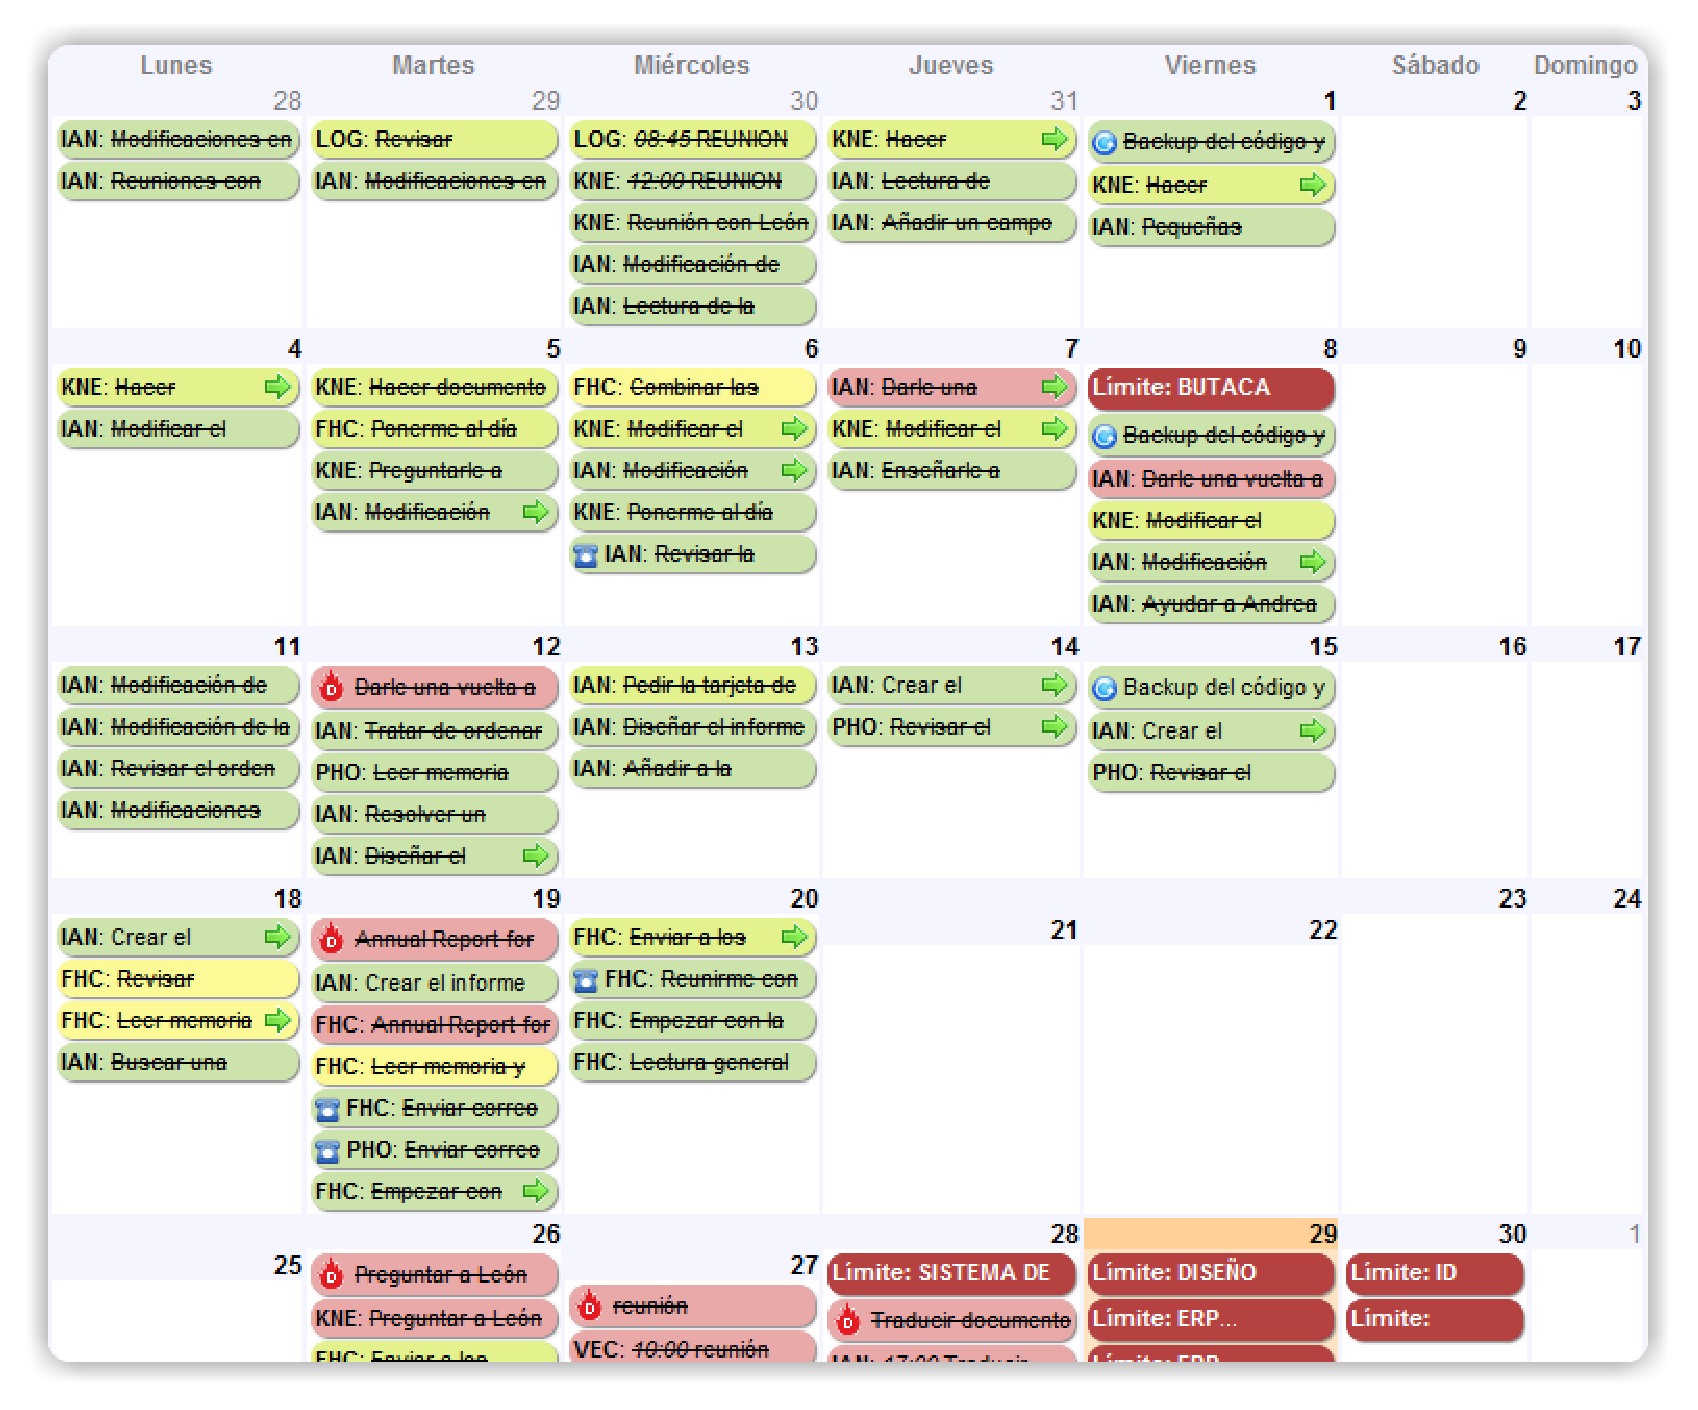
\epsfig{file=imagenes/otrosproyectos/tareas_cal2.eps,height=5in,angle=90}
\caption{Vista de calendario del gestor del tiempo.}
\label{fig:tareas_cal2}
\end{figure}

\begin{figure}
\centering
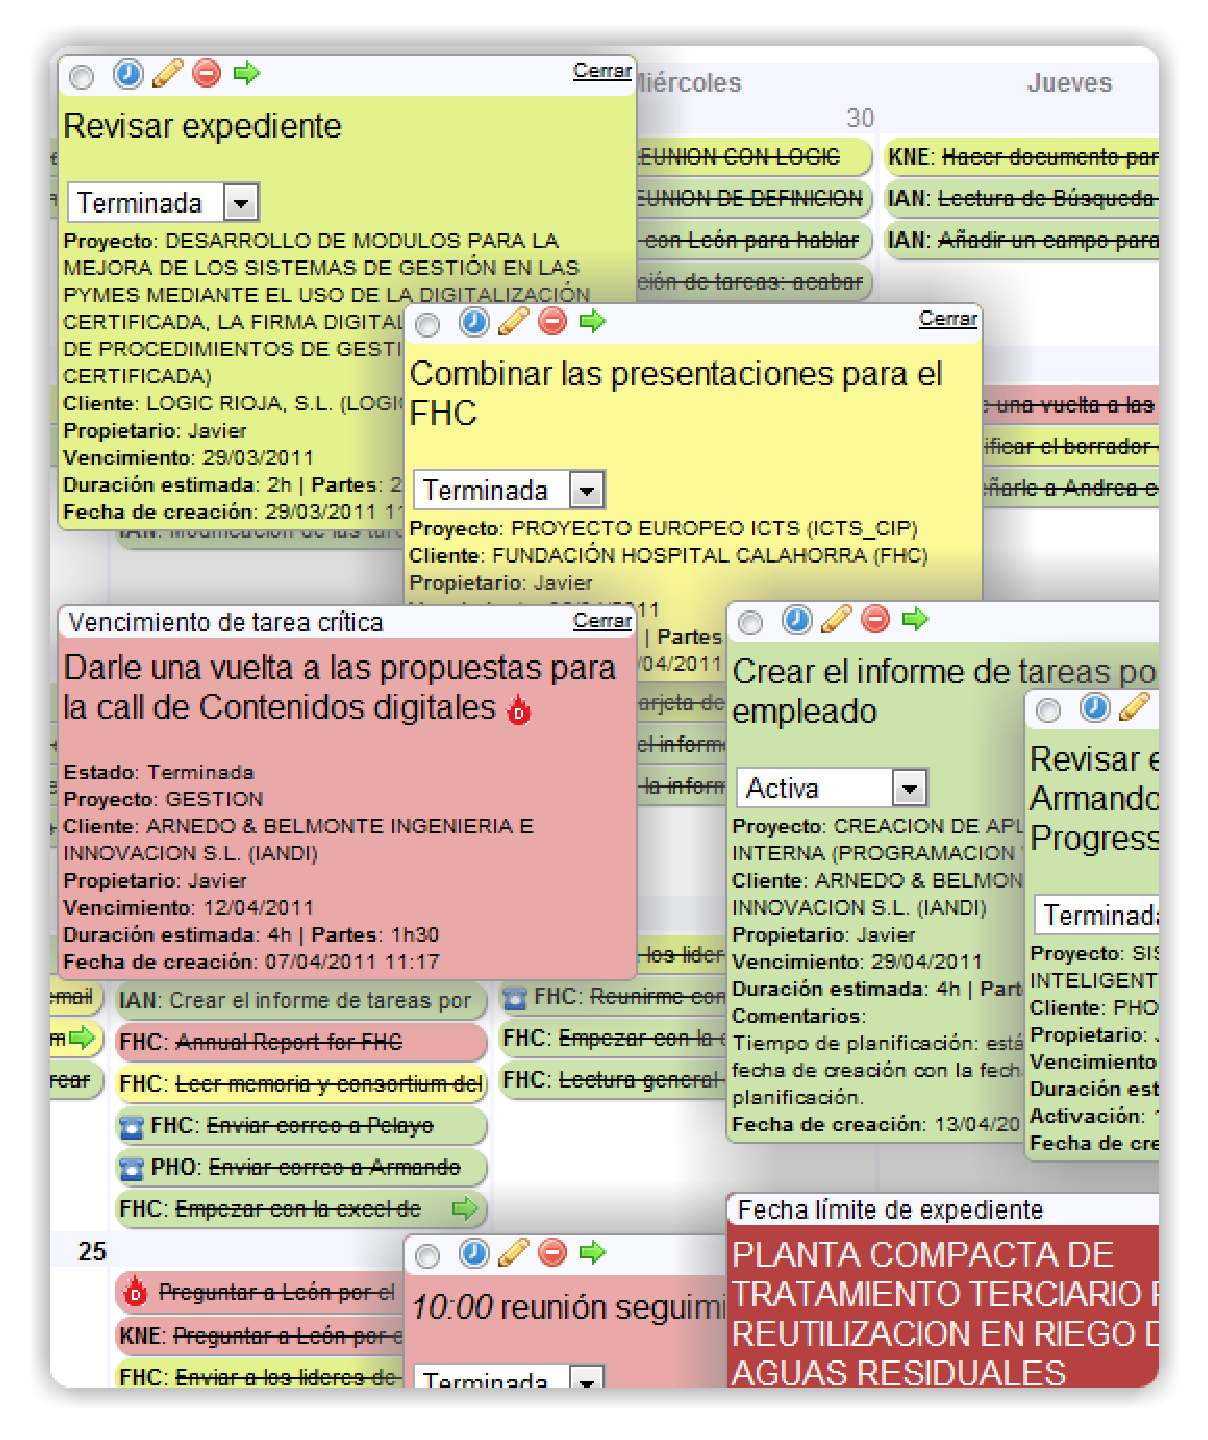
\epsfig{file=imagenes/otrosproyectos/tareas2.eps,width=5in}
\caption{Detalle de las tareas del calendario.}
\label{fig:tareas2}
\end{figure}

\begin{figure}
\centering
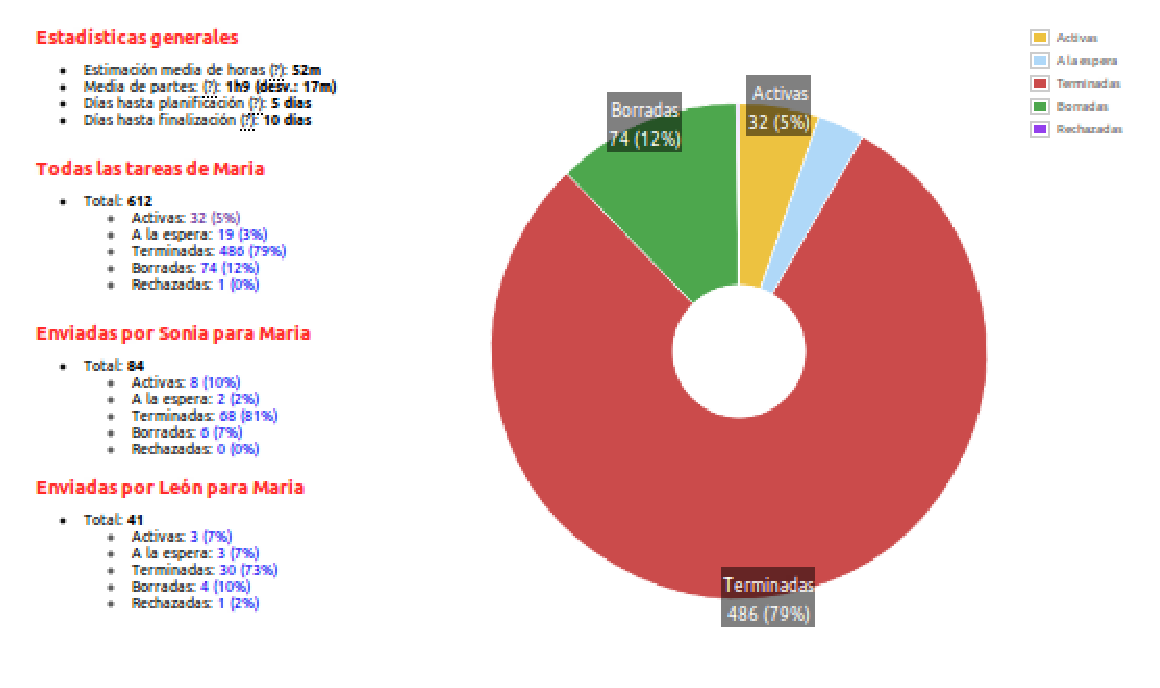
\epsfig{file=imagenes/otrosproyectos/tareas_stats.eps,width=5in}
\caption{Estadísticas de tareas.}
\label{fig:tareas_stats}
\end{figure}

\begin{figure}
\centering
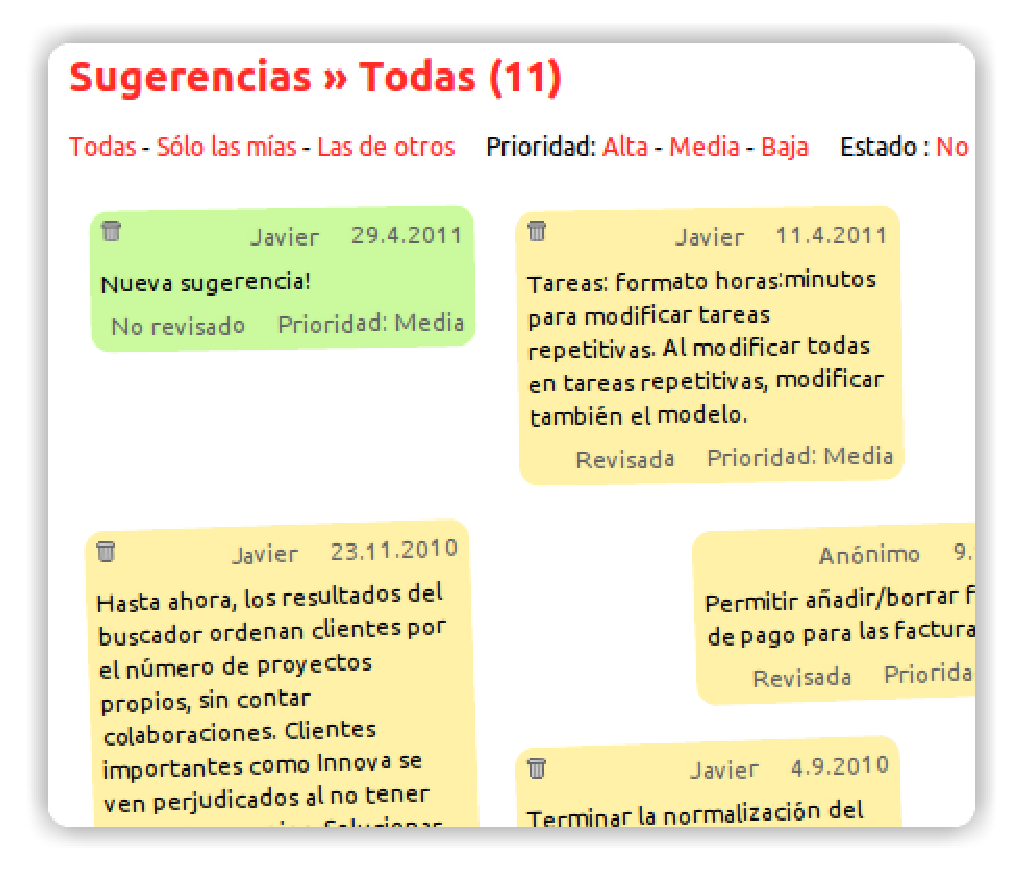
\epsfig{file=imagenes/otrosproyectos/sugerencias.eps,width=4in}
\caption{Sistema de sugerencias.}
\label{fig:sugerencias}
\end{figure}

\begin{figure}
\centering
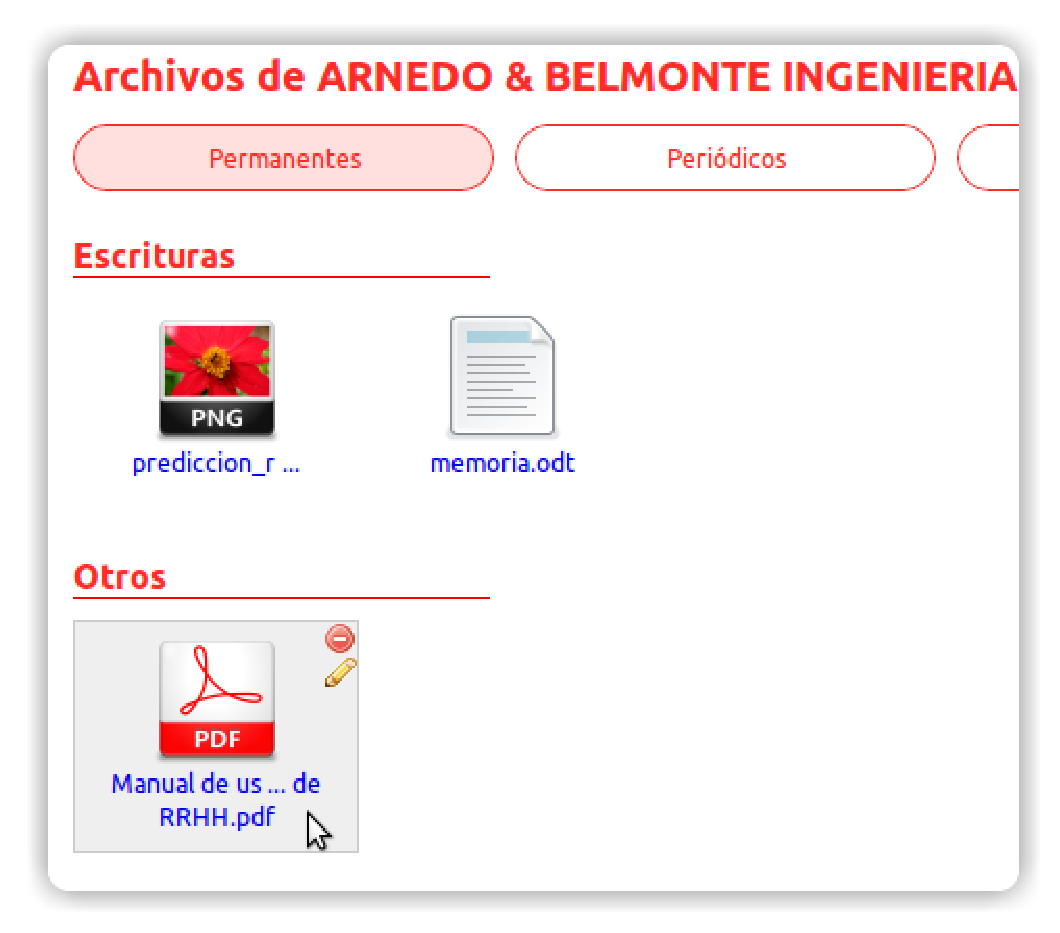
\epsfig{file=imagenes/otrosproyectos/archivos.eps,width=3.5in}
\caption{Gestor de archivos.}
\label{fig:archivos}
\end{figure}


\begin{figure}
\centering
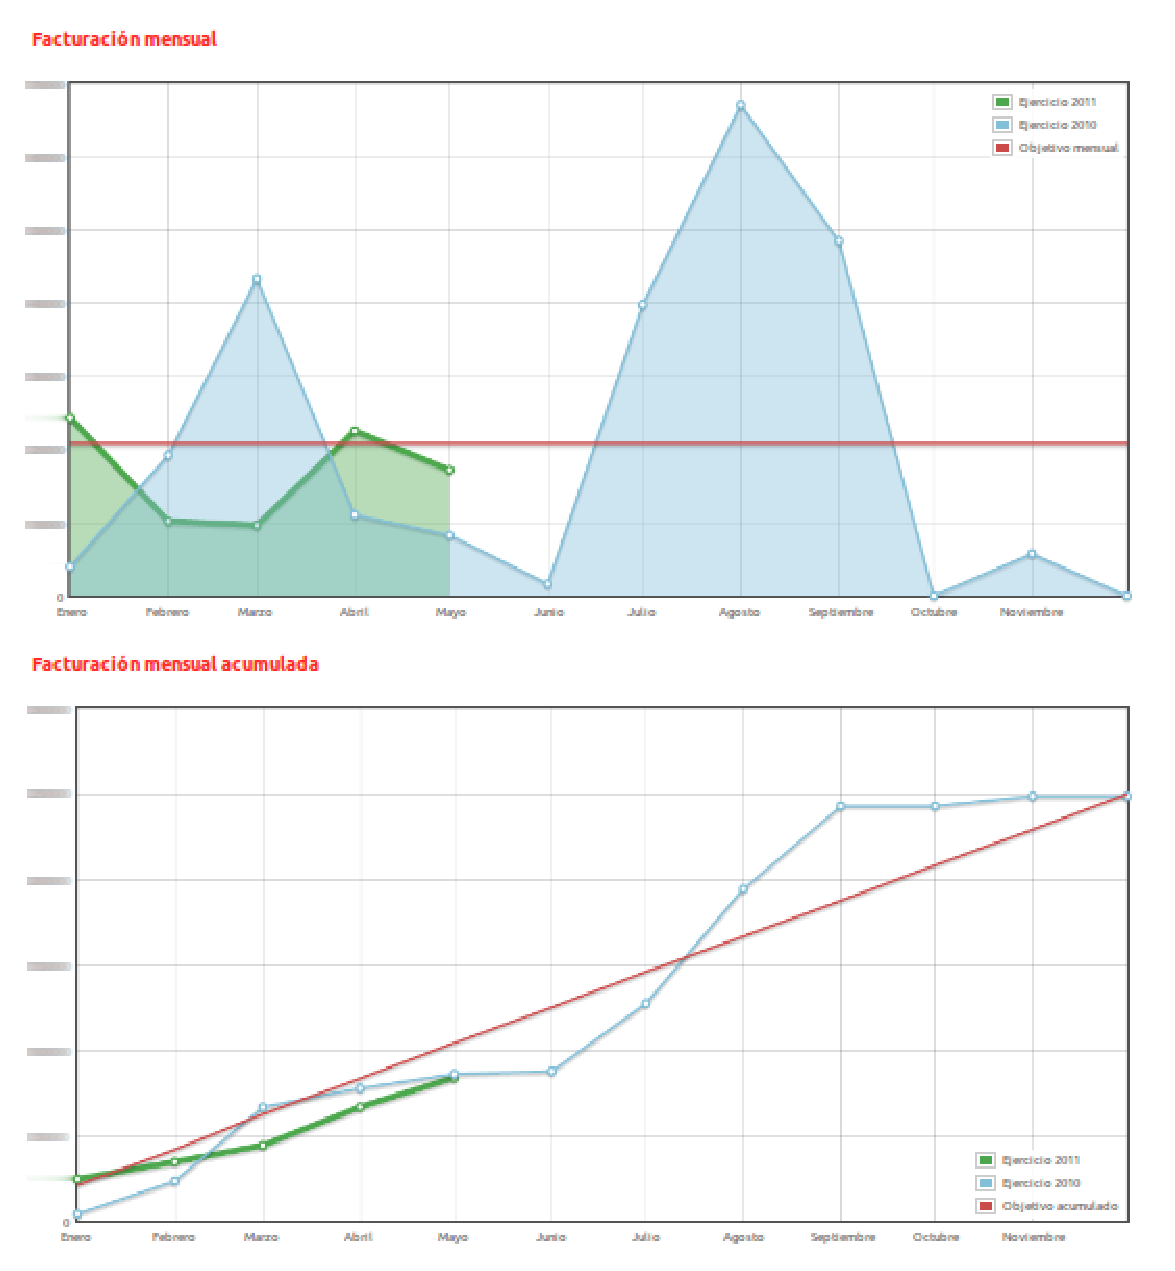
\epsfig{file=imagenes/otrosproyectos/facturacion.eps,width=3.5in}
\caption{Facturación comparada mensual (arriba) y acumulada.}
\label{fig:facturacion}
\end{figure}
